% =============================================================
% Árbol de decisión para calificar BCS desde atrás (figura del paper).
% Dos filas horizontales: grupa en V (vacas flacas, hojas arriba) y grupa en U
% (vacas gordas, hojas abajo). Pensado para el ancho de dos columnas.
% Compilar: pdflatex arbol_bcs.tex  ->  arbol_bcs.pdf
% =============================================================
\documentclass[tikz,border=3pt]{standalone}
\usepackage[utf8]{inputenc}
\usepackage[T1]{fontenc}
\usetikzlibrary{arrows.meta,positioning,calc}

% hojas coloreadas del azul (flaca) al rojo (gorda), como los mapas de calor
\definecolor{b200}{HTML}{6BAED6}\definecolor{b225}{HTML}{8DC0DF}\definecolor{b250}{HTML}{A9CFE6}
\definecolor{b275}{HTML}{C6DEEE}\definecolor{b300}{HTML}{E1ECF4}\definecolor{b325}{HTML}{F2F2F2}
\definecolor{b350}{HTML}{F8E3DA}\definecolor{b375}{HTML}{F6CFBE}\definecolor{b400}{HTML}{F3BBA3}
\definecolor{b425}{HTML}{EFA488}\definecolor{b450}{HTML}{E98D6E}\definecolor{b475}{HTML}{E07656}
\definecolor{b500}{HTML}{D45F43}
\definecolor{preg}{HTML}{EEF0FA}\definecolor{borde}{HTML}{6B6FA8}

\tikzset{
  font=\sffamily\scriptsize, >={Stealth[length=1.6mm]},
  q/.style={draw=borde, fill=preg, rounded corners=5pt, line width=0.5pt, align=center,
            text width=1.66cm, minimum height=0.95cm, inner sep=2pt},
  hoja/.style={draw=black!55, line width=0.4pt, fill=#1, align=center, minimum width=1.25cm,
               minimum height=0.48cm, inner sep=1.5pt, font=\sffamily\scriptsize\bfseries},
  a/.style={->, line width=0.5pt, draw=black!70},
  et/.style={font=\sffamily\tiny, fill=white, inner sep=1pt},
}

\begin{document}
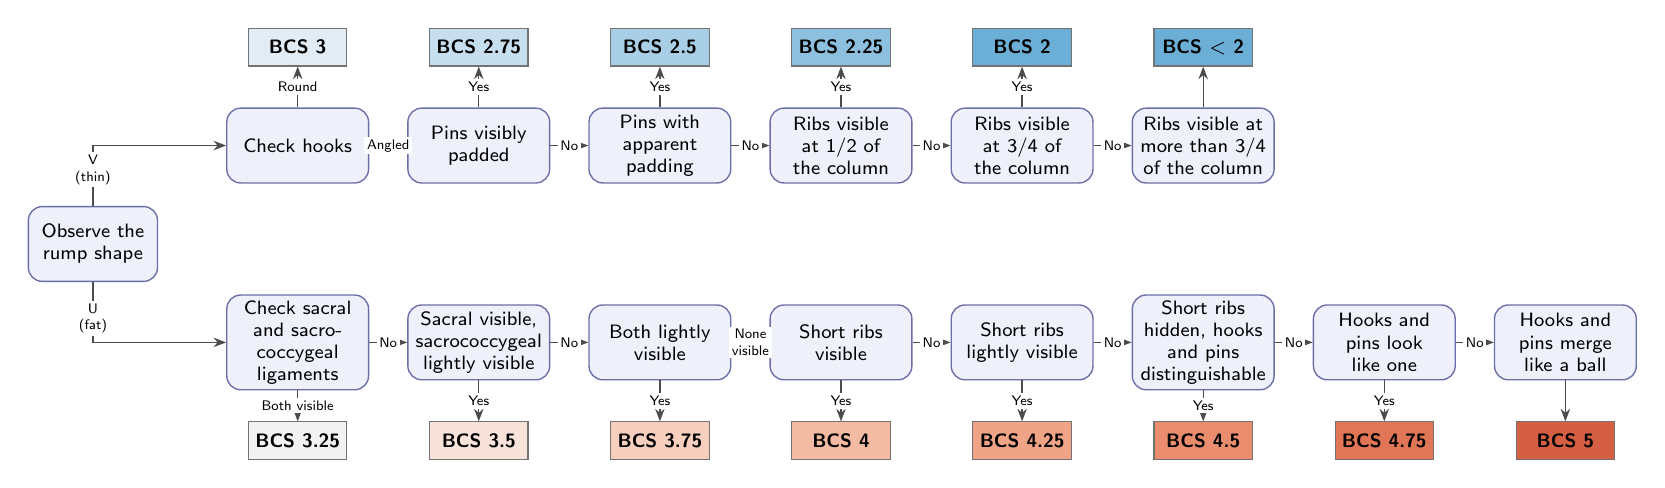
\begin{tikzpicture}
  \def\dx{2.3}            % separación horizontal entre preguntas
  \def\yv{1.25}\def\yu{-1.25}\def\h{1.25}

  % raíz
  \node[q, text width=1.5cm] (A) at (0,0) {Observe the rump shape};

  % ---------- grupa en V (fila de arriba, hojas encima) ----------
  \node[q] (B) at (1*\dx+0.3,\yv) {Check hooks};
  \node[q] (D) at (2*\dx+0.3,\yv) {Pins visibly padded};
  \node[q] (F) at (3*\dx+0.3,\yv) {Pins with apparent padding};
  \node[q] (G) at (4*\dx+0.3,\yv) {Ribs visible at 1/2 of the column};
  \node[q] (H) at (5*\dx+0.3,\yv) {Ribs visible at 3/4 of the column};
  \node[q] (I) at (6*\dx+0.3,\yv) {Ribs visible at more than 3/4 of the column};
  \node[hoja=b300] (s300) at ($(B)+(0,\h)$) {BCS 3};
  \node[hoja=b275] (s275) at ($(D)+(0,\h)$) {BCS 2.75};
  \node[hoja=b250] (s250) at ($(F)+(0,\h)$) {BCS 2.5};
  \node[hoja=b225] (s225) at ($(G)+(0,\h)$) {BCS 2.25};
  \node[hoja=b200] (s200) at ($(H)+(0,\h)$) {BCS 2};
  \node[hoja=b200] (s199) at ($(I)+(0,\h)$) {BCS $<$ 2};
  \draw[a] (A.north) |- node[et, pos=0.3, align=center] {V\\(thin)} (B.west);
  \draw[a] (B) -- node[et] {Angled} (D);
  \draw[a] (D) -- node[et] {No} (F);
  \draw[a] (F) -- node[et] {No} (G);
  \draw[a] (G) -- node[et] {No} (H);
  \draw[a] (H) -- node[et] {No} (I);
  \draw[a] (B) -- node[et] {Round} (s300);
  \draw[a] (D) -- node[et] {Yes} (s275);
  \draw[a] (F) -- node[et] {Yes} (s250);
  \draw[a] (G) -- node[et] {Yes} (s225);
  \draw[a] (H) -- node[et] {Yes} (s200);
  \draw[a] (I) -- (s199);

  % ---------- grupa en U (fila de abajo, hojas debajo) ----------
  \node[q] (C) at (1*\dx+0.3,\yu) {Check sacral and sacro\-coccygeal ligaments};
  \node[q] (J) at (2*\dx+0.3,\yu) {Sacral visible, sacro\-coccygeal lightly visible};
  \node[q] (K) at (3*\dx+0.3,\yu) {Both lightly visible};
  \node[q] (M) at (4*\dx+0.3,\yu) {Short ribs visible};
  \node[q] (N) at (5*\dx+0.3,\yu) {Short ribs lightly visible};
  \node[q] (O) at (6*\dx+0.3,\yu) {Short ribs hidden, hooks and pins distinguishable};
  \node[q] (P) at (7*\dx+0.3,\yu) {Hooks and pins look like one};
  \node[q] (Q) at (8*\dx+0.3,\yu) {Hooks and pins merge like a ball};
  \node[hoja=b325] (s325) at ($(C)-(0,\h)$) {BCS 3.25};
  \node[hoja=b350] (s350) at ($(J)-(0,\h)$) {BCS 3.5};
  \node[hoja=b375] (s375) at ($(K)-(0,\h)$) {BCS 3.75};
  \node[hoja=b400] (s400) at ($(M)-(0,\h)$) {BCS 4};
  \node[hoja=b425] (s425) at ($(N)-(0,\h)$) {BCS 4.25};
  \node[hoja=b450] (s450) at ($(O)-(0,\h)$) {BCS 4.5};
  \node[hoja=b475] (s475) at ($(P)-(0,\h)$) {BCS 4.75};
  \node[hoja=b500] (s500) at ($(Q)-(0,\h)$) {BCS 5};
  \draw[a] (A.south) |- node[et, pos=0.3, align=center] {U\\(fat)} (C.west);
  \draw[a] (C) -- node[et] {No} (J);
  \draw[a] (J) -- node[et] {No} (K);
  \draw[a] (K) -- node[et, align=center] {None\\visible} (M);
  \draw[a] (M) -- node[et] {No} (N);
  \draw[a] (N) -- node[et] {No} (O);
  \draw[a] (O) -- node[et] {No} (P);
  \draw[a] (P) -- node[et] {No} (Q);
  \draw[a] (C) -- node[et] {Both visible} (s325);
  \draw[a] (J) -- node[et] {Yes} (s350);
  \draw[a] (K) -- node[et] {Yes} (s375);
  \draw[a] (M) -- node[et] {Yes} (s400);
  \draw[a] (N) -- node[et] {Yes} (s425);
  \draw[a] (O) -- node[et] {Yes} (s450);
  \draw[a] (P) -- node[et] {Yes} (s475);
  \draw[a] (Q) -- (s500);

\end{tikzpicture}
\end{document}
